\documentclass[tikz,border=2pt]{standalone}
\usepackage{amsmath,amssymb}
\usepackage{tikz}
\usetikzlibrary{arrows.meta}

\begin{document}
% The sum of two planes through the origin in R^3 is all of R^3; their intersection is a line,
% so the decomposition w = v1 + v2 is not unique (the sum is not direct).
% Explicit spatial model: V1=span(e1,e2), V2=span(e1,e3), intersection=span(e1).
% Use one linear projection for the planes, axes and common line.
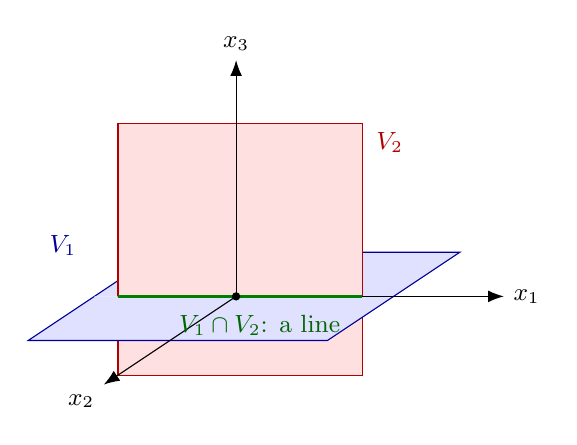
\begin{tikzpicture}[every node/.style={font=\small}, >={Latex[length=2mm]},
    x={(1cm,0cm)}, y={(-0.6cm,-0.4cm)}, z={(0cm,1cm)}]
    % Draw order gives the occlusion for a view from above and in front: back half of V1 (x2<0), V2, front half of V1 (x2>0), then axes and common line.
    \fill[blue!12] (-1.8,-1.4,0) -- (2,-1.4,0) -- (2,0,0) -- (-1.8,0,0) -- cycle;
    \draw[blue!60!black] (-1.8,0,0) -- (-1.8,-1.4,0) -- (2,-1.4,0) -- (2,0,0);
    \filldraw[fill=red!12,draw=red!70!black] (-1.5,0,-1.0) -- (1.6,0,-1.0) -- (1.6,0,2.2) -- (-1.5,0,2.2) -- cycle;
    \fill[blue!12] (-1.8,0,0) -- (2,0,0) -- (2,1.4,0) -- (-1.8,1.4,0) -- cycle;
    \draw[blue!60!black] (2,0,0) -- (2,1.4,0) -- (-1.8,1.4,0) -- (-1.8,0,0);
    \draw[->] (0,0,0) -- (3.4,0,0) node[right] {$x_1$};
    \draw[->] (0,0,0) -- (0,0,3.0) node[above] {$x_3$};
    \draw[->] (0,0,0) -- (0,2.8,0) node[below left] {$x_2$};
    \draw[green!50!black,very thick] (-1.5,0,0) -- (1.6,0,0);
    \node[blue!60!black,font=\small] at (-2.2,0,0.65) {$V_1$};
    \node[red!70!black,font=\small] at (1.95,0,1.95) {$V_2$};
    \node[green!40!black,font=\small,anchor=north] at (0.3,0,-0.12) {$V_1\cap V_2$: a line};
    \fill (0,0,0) circle (1.5pt);
\end{tikzpicture}
\end{document}
